% This must be in the first 5 lines to tell arXiv to use pdfLaTeX, which is strongly recommended.
\pdfoutput=1
% In particular, the hyperref package requires pdfLaTeX in order to break URLs across lines.

\documentclass[11pt,table,xcdraw]{article}

% Remove the "guidelines" option to generate the final version.
%\usepackage[guidelines]{nlpreport} % show guidelines
\usepackage[]{nlpreport} % hide guidelines


% Standard package includes
\usepackage{times}
\usepackage{latexsym}

% For proper rendering and hyphenation of words containing Latin characters (including in bib files)
\usepackage[T1]{fontenc}
% For Vietnamese characters
% \usepackage[T5]{fontenc}
% See https://www.latex-project.org/help/documentation/encguide.pdf for other character sets

% This assumes your files are encoded as UTF8
\usepackage[utf8]{inputenc}

% This is not strictly necessary, and may be commented out,
% but it will improve the layout of the manuscript,
% and will typically save some space.
\usepackage{microtype}
\usepackage{graphicx}
\usepackage{hyperref}
\usepackage{amsmath}
\usepackage{mathtools}
\usepackage{multirow}
\usepackage{listings}
\usepackage{xcolor}
\usepackage{booktabs} % for tables
\usepackage{todonotes} % for todos...

% THE pdfinfo Title AND Author ARE NOT NECESSARY, THEY ARE METADATA FOR THE FINAL PDF FILE
\hypersetup{pdfinfo={
Title={SemEval 2024 Task 10: Emotion Discovery and Reasoning its Flip in Conversation (EDiReF)},
Author={
    Daniel Bernardi,
    Daniele Santini,
    Hiari Pizzini Cavagna
    \&
    Muhammad Saleem Ghulam
}
}}
%\setcounter{secnumdepth}{0}  
 \begin{document}
%
\title{SemEval 2024 Task 10: Emotion Discovery and Reasoning its Flip in Conversation (EDiReF)\\
\explanation{\rm Substitute the $\uparrow$ title $\uparrow$ with your project's title, or with Assignment 1 / 2\\ \smallskip}
% subtitle:
\large \explanation{\rm $\downarrow$ Keep only one of the following three  labels  / leave empty for assignments: $\downarrow$\\}
NLP Course Project
}
\author{
    Daniel Bernardi,
    Daniele Santini,
    Hiari Pizzini Cavagna
    \and
    Muhammad Saleem Ghulam\\
Master's Degree in Artificial Intelligence, University of Bologna\\
\{ daniel.bernardi, daniele.santini2, hiari.pizzinicavagna, muhammad.ghulam \}@studio.unibo.it
}
\maketitle


\attention{DO NOT MODIFY THIS TEMPLATE - EXCEPT, OF COURSE FOR TITLE, SUBTITLE AND AUTHORS.\\ IN THE FINAL VERSION, IN THE \LaTeX\ SOURCE REMOVE THE \texttt{guidelines} OPTION FROM  \texttt{$\backslash$usepackage[guidelines]\{nlpreport\}}.
}

\begin{abstract}
We challenged the SemEval task about Emotion Recognition (ERC) and Emotion Flip Reasoning (EFR) in English Conversations. For this task, a system should be able to classify the emotion of each sentence and if that sentence caused an emotion flip in the conversation.
We developed a PyTorch model based on BERT for both emotion and trigger prediction. 
The proposed solution demonstrates promising performance in the ERC task. However, its performance on the EFR task is not good enough. 
To make an attempt in overcoming the emotion flips detection problems, we tried to balance the training set by using a WeightedSampler, or to increase the weight of the trigger prediction in the loss function. Another tentative for balancing the dataset was based on the Easy Data Augmentation approach, by using the \textit{nlpaug} library. These solutions didn't improve the overall performance of the model as expected. An input encoding with more context, however, gave a small performance improvement.


%\begin{quote}
\explanation{
The abstract is very brief summary of your report. Try to keep it no longer than 15-20 lines at most. Write your objective, your approach, and your main observations (what are the findings that make this report worthwhile reading?)}

%\end{quote}

\end{abstract}

\attention{\textcolor{red}{NOTICE: THIS REPORT'S LENGTH MUST RESPECT THE FOLLOWING PAGE LIMITS: \begin{itemize}
    \item ASSIGNMENT: \textbf{2 PAGES} 
    \item NLP PROJECT OR PROJECT WORK: \textbf{8 PAGES}
    \item COMBINED NLP PROJECT + PW: \textbf{12 PAGES}
\end{itemize}  PLUS LINKS, REFERENCES AND APPENDICES.\\ 
THIS MEANS THAT YOU CANNOT FILL ALL SECTIONS TO MAXIMUM LENGTH. IT ALSO MEANS THAT, QUITE POSSIBLY, YOU WILL HAVE TO LEAVE OUT OF THE REPORT PART OF THE WORK YOU HAVE DONE OR OBSERVATIONS YOU HAVE. THIS IS NORMAL: THE REPORT SHOULD EMPHASIZE WHAT IS MOST SIGNIFICANT, NOTEWORTHY, AND REFER TO THE NOTEBOOK FOR ANYTHING ELSE.\\ 
FOR ANY OTHER ASPECT OF YOUR WORK THAT YOU WOULD LIKE TO EMPHASIZE BUT CANNOT EXPLAIN HERE FOR LACK OF SPACE, FEEL FREE TO ADD COMMENTS IN THE NOTEBOOK.\\ 
INTERESTING TEXT EXAMPLES THAT EXCEED THE MAXIMUM LENGTH OF THE REPORT CAN BE PLACED IN A DEDICATED APPENDIX AFTER THE REFERENCES.}}


\section{Introduction}
\label{sec:introduction}
Here is a brief description of the two tasks that need to be tackled. 

The Emotion Recognition in Conversation (ERC) task is defined as follows: given a dialogue, ERC aims to assign an emotion to each utterance from a predefined set of possible emotions. Seven emotions were defined for this task: \textit{neutral}, \textit{joy}, \textit{sadness}, \textit{surprise}, \textit{disgust}, \textit{anger} and \textit{fear}.

The Emotion Flip Reasoning task is defined as follows: given a dialogue, EFR aims to identify the trigger utterance(s) for an emotion-flip in a multi-party conversation dialogue. The task of recognizing an emotion-flip is not trivial. Let's suppose that two people $S_1$ and $S_2$ are involved in the conversation and that we're analyzing an utterance pronounced by $S_2$. To grasp the eventful presence of an emotion-flip there is need to comprehend and link the emotions of the previous and future sentences.

The importance of these tasks stands in the ability of a Digital System to understand sentences' emotions, and how sentences can drive the course of the dialogue. Digital Systems are becoming more powerful and useful day after day, and are now used for both professional and personal tasks, especially after the recent advances on LLMs. An example of how such a system could be useful can be taken by the videogame \textit{Detroit: Become Human}. The scope of the game is for the player to take actions in a futuristic but realistic simulation of our World. The main characters are Androids, deeply integrated the society because of their humanoid shape and thinking. The Androids usually interact with humans, which could be violent, alterated or sad, and the conversation development may change drastically based on the Android responses. Even if we're stretching the reality and entering the fictional world, for those Androids, a much more evolved ERC and EFR system could be fundamental to understand emotions and the dialogue's development. Another possible use case would be for Police Forces, which could make use of such a system to verbally interact in the safest way during problematic situations. 

Emotion Recognition is a task similar to Sentiment Analysis, which is not new in the Natural Language Processing world. Many systems were developed to solve these tasks. Usually, the crucial point is to understand emotions based on word usage and meaning. If the solution requires to understand deeply a sentence, Language Models (e.g. Transformers based LMs) may provide a powerful, generic and good solution.

On the contrary, an EFR system cannot base its answer on a single sentence. In fact, being able to understand if the emotion changes in a dialogue requires a system that perceives the evolution of the emotions, sentence-by-sentence. The previous and future context of a sentence gains crucial importance. A transformer based solution seems required.

Our approach to solve the task is to fine-tune a BERT model \cite{devlin2019bert} with two classification heads, which give the model the ability to output both an emotion and the trigger value for each sentence of a dialogue, as by project's guidelines. More specifically, we use a pre-trained BERT checkpoint (bert-base-uncased) as the main module of our model. After some experiments and online research, we decided to concatenate the last 4 hidden layers' outputs as input for our linear classification layers. Since the BERT checkpoint was trained for the Next-Sentence Prediction task, we decided to create an input for each dialogue's sentence, by defining the current sentence, the next, and the previous sentence(s) (the history). Our inputs for BERT are a concatenation of these texts, which provide the necessary context for the two tasks.

The two BERT setups, freezed base-model and Fully finetuned model, were tested on four different configurations. The goal was to try improving the performance of the baseline, more specifically for the EFR task. One of those configuration was standard, while the others included the use of a Weighted Sampler to balance the dataset (trigger-wise), or a loss calculation that enhanced the importance of correct trigger predictions, or the use of the \textit{nlpaug} library to augment the training set, increasing the support of emotion flips. 

At the end of these experiments we concluded that these solution could not result in a model with better overall performances. Instead, we obtained the best improvements by giving more textual context to the BERT model.


\attention{MAX 1 COLUMN FOR ASSIGNMENT REPORTS / 2 COLUMNS FOR PROJECT OR PW / 3 FOR COMBINED REPORTS.}

\explanation{
The Introduction is an executive summary, which you can think of as an extended abstract.  Start by writing a brief description of the problem you are tackling and why it is important. (Skip it if this is an assignment report).} 

\explanation{Then give a short overview of known/standard/possible approaches to that problems, if any, and what are their advantages/limitations.} 

\explanation{After that, discuss your approach, and motivate why you follow that approach. If you are drawing inspiration from an existing model, study, paper, textbook example, challenge, \dots, be sure to add all the necessary references~\cite{DBLP:journals/corr/abs-2204-02311,DBLP:conf/acl/LorenzoMN22,DBLP:conf/clef/AnticiBIIGR21,DBLP:conf/ijcai/NakovCHAEBPSM21,DBLP:conf/naacl/RottgerVHP22,DBLP:journals/toit/LippiT16}.\footnote{\href{https://en.wikipedia.org/wiki/The_Muppet_Show}{Add only what is relevant.}}}

\explanation{Next, give a brief summary of your experimental setup: how many experiments did you run on which dataset. Last, make a list of the main results or take-home lessons from your work.}

\attention{HERE AND EVERYWHERE ELSE: ALWAYS KEEP IN MIND THAT, CRUCIALLY, WHATEVER TEXT/CODE/FIGURES/IDEAS/... YOU TAKE FROM ELSEWHERE MUST BE CLEARLY IDENTIFIED AND PROPERLY REFERENCED IN THE REPORT.}




\section{Background}
\label{sec:background}

\subsection{Weighted Sampler} \label{weighted_sampler}
The WeightedSampler is a PyTorch class. More specifically, it is a sampler utilized by a DataLoader to extract inputs from a dataset. It is possible to specify, for each input row, its probability to be extracted. This provides a solution to the imbalanced nature of some datasets. For the EFR task we tried this approach by enhancing the emotion flipping sentences' probability to get extracted.

\subsection{Easy Data Augmentation}
Easy Data Augmentation \cite{wei2019eda} is an approach for the augmentation of textual datasets. The augmentation is based on the elaboration of sentences at word-level, with operations of random \textit{synonym replacement}, \textit{insertion}, \textit{removal} and \textit{swap}.

\subsection{nlpaug} \label{nlpaug}
The \textit{nlpaug} library \cite{ma2019nlpaug} implements many classes for data augmentation of textual and audio sources. It is possible to do operations on Characters, Words and Sentences.

\paragraph{Contextual Word Embeddings Augmenter}
Augmenter that leverage contextual word embeddings to find top n similar word for augmentation. It can be used to implement the Easy Data Augmentation's approach while making use of a model such as BERT.

\attention{MAX 2 COLUMNS (3 FOR COMBINED REPORTS). DO NOT INCLUDE SECTION IF NO BACKGROUND NECESSARY. OMIT SECTION IN ASSIGNMENT REPORTS.}

\explanation{The Background section is where you briefly provide whatever background information on the domain or challenge you're addressing and/or on the techniques/approaches you're using, that (1) you think is necessary for the reader to understand your work and design choices, and (2) is not something that has been explained to you during the NLP course (to be clear: do NOT repeat explanations of things seen in class, we already know that stuff). If you adapt paragraphs from articles, books, online resources, etc: be sure to clarify which parts are yours and which ones aren't.}


\section{System description}
\label{sec:system}
The loading and the processing of the dataset is done by using the Pandas library. A Label Encoder from scikit-learn is used to convert the emotion labels from categorical data into numerical representations. We have implemented and trained the model using the PyTorch library. The HuggingFace Transformers library provides the necessary tools to encode the data, and also to load and train the pre-trained BERT model. A pre-trained Tokenizer and a pre-trained Model are loaded from the library using the \textit{bert-base-uncased} checkpoint.\\

We utilized the dataset provided by SemEval, which contains different conversations, and each of them is labeled with a list of emotions, each for each utterance, and a list of binary triggers, that indicates if the utterance triggers an emotion flip inside the dialogue. After the loading, the initial step is the pre-processing of the data. For processing, encoding and training reasons we decided to decompose the dialogues into single utterance, and assigning them to their corresponding labels for emotion and trigger. Furthermore for each utterance we added two additional features, the history and the future, containing respectively previous two sentences and one next sentence of the same dialogue. These additional features are required for a better understanding of the context during training by the model, in a way to improve the overall performance.
After the pre-processing and splitting, the input data is encoded using the Tokenizer, by concatenating history, utterance and future features, and then each input sequence is converted into a sequence of tokens \textit{([CLS] history+utterance [SEP] future-utterance)}. The PyTorch Dataset and Dataloader are used to prepare the encoded data for the training.\\

We implemented a transformer-based model, specifically the pre-trained BERT (Bidirectional Encoder Representations from Transformers). A fine-tuning process is implemented to adapt the BERT model to our specific tasks, by adding a classification head on top of the BERT architecture. As we want to predict two features, we are performing a multi-task-learning, by sharing the pre-trained BERT base layers and a Linear layer, and then feeding separate classification heads for each task. In our case the output of BERT architecture is passed through a Linear layer,  and then we have the following two streams:
\begin{itemize}
    \item For the prediction of emotions, we have a Tanh function, a Dropout layer and a Linear layer followed by a Softmax function (in PyTorch is incorporated in the CrossEntropyLoss). As just mentioned the criterion for computing the loss is the CrossEntropyLoss ;
    \item For the prediction of triggers, we have a ReLU Function, a Dropout layer and a Sigmoid function on a single output of a Linear layer. In this case the loss is computed by using the BinaryCrossEntropy criterion.
\end{itemize}
An implementation of the network heads is shown in \autoref{fig:cls_model}.\\
 
BERT produces different outputs that can be used for classification tasks, such as the pooler output, the sequence output and the hidden states. The pooler output contains a summary representation of the sequence, and it's basically the [CLS] token of the last hidden state passed through a linear layer with a non linear activation function. The sequence output contains an embedding for each token in the input sequence. Instead the hidden states refer to the outputs of each layer of BERT, by making possible to aggregate information from multiple layers. There are different configurations that can be used depending on the tasks, after some experimentation we decided to take the mean between the [CLS] tokens of the last four hidden states, and feed the top layers. In our case this configuration turns out to perform slightly better than other alternatives, such as the pooler outptut or the concatenation of the last four hidden states.\\

\attention{MAX 1 COLUMN FOR ASSIGNMENT REPORTS / 4 COLUMNS FOR PROJECT OR PW / 6 FOR COMBINED REPORTS.}

\explanation{
Describe the system or systems you have implemented (architectures, pipelines, etc), and used to run your experiments. If you reuse parts of code written by others, be sure to make very clear your original contribution in terms of
\begin{itemize}
    \item architecture: is the architecture your design or did you take it from somewhere else
    \item coding: which parts of code are original or heavily adapted? adapted from existing sources? taken from external sources with minimal adaptations?
\end{itemize}
It is a good idea to add figures to illustrate your pipeline and/or architecture(s)
(see Figure~\ref{fig:architecture})
%
\begin{figure*}
    \centering
    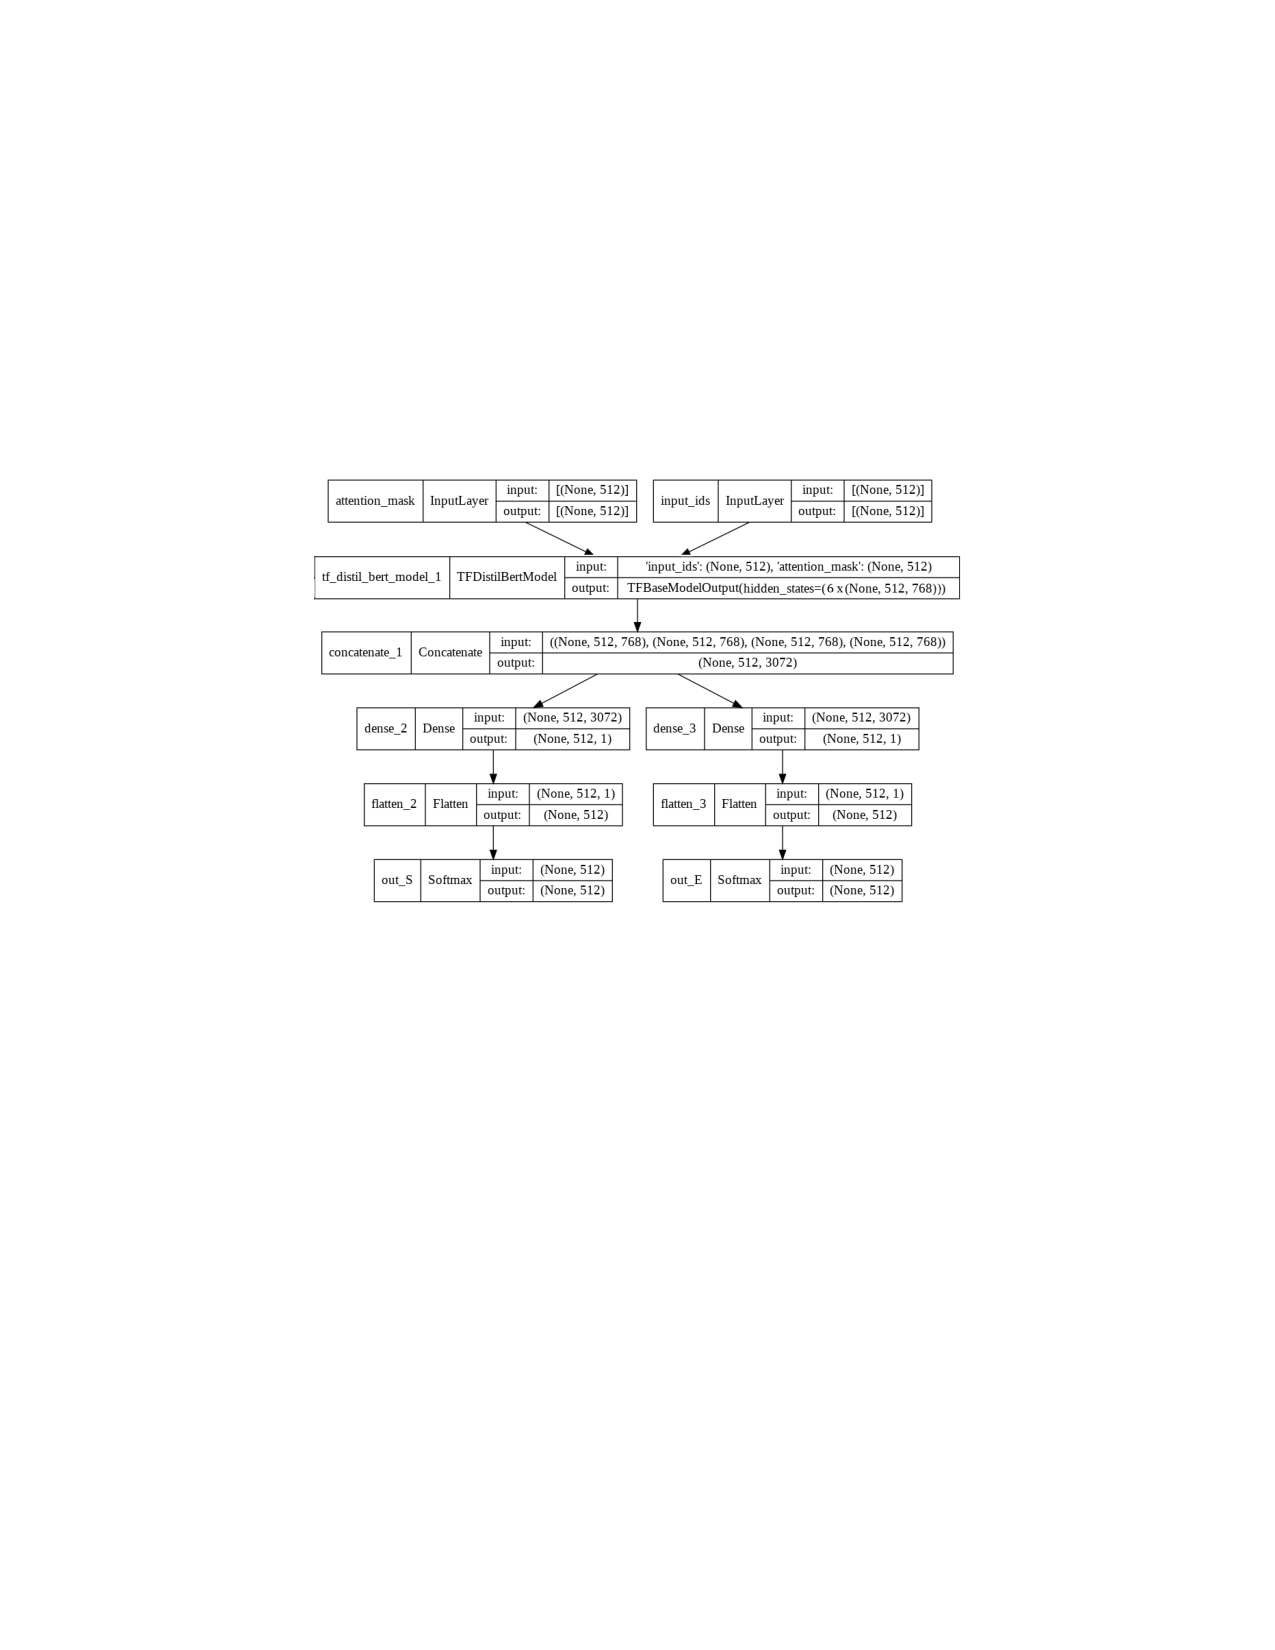
\includegraphics[width=\textwidth]{img/architecture.pdf}
    \caption{Model architecture}
    \label{fig:architecture}
\end{figure*}
}

\begin{figure*}
    \centering
    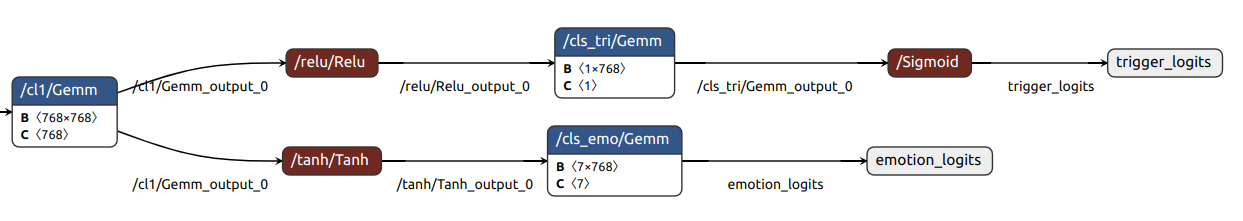
\includegraphics[width=\textwidth]{img/heads.png}
    \caption{Classification heads implementation on the top of BERT.}
    \label{fig:cls_model}
\end{figure*}



\section{Data}
\label{sec:data}

The data used in this project was given by SemEval and is freely accessible online, the link is provided in Section~\ref{sec:links}. The data is formatted as a list of dictionaries, each of them containing 5 keys: \textit{episode, speakers, emotions, utterances, triggers}. The utterances value contains the dialogue between the speakers in a list format, splitted at the sentence level. The emotions and the triggers values are the labels used for the classification tasks, respectively string labels and float labels (0.0 or 1.0). 

The data is loaded into a Pandas DataFrame and splitted in training, validation and test sets.
The pre-processing steps we followed are the following:
\begin{itemize}
    \item Substitution of wrongly-loaded trigger values, from \textit{None} to \textit{0.0}.
    \item trigger label formatted as boolean values.
    \item dropped the \textit{speakers} column.
    \item after performing the data split into training, validation and test set, we splitted each \textit{episode}, creating a row in the DataFrames for each utterance of a dialogue.
    \item created the \textit{history} and the \textit{future} columns. The former included a concatenation of two previous sentences of the utterance, the latter contained the next sentence.
\end{itemize}

Some analysis on the distribution of data showed that the distribution of emotion classes is imbalanced (see Figure \ref{fig:em_dist}). 
\begin{figure}[]
    \centering
    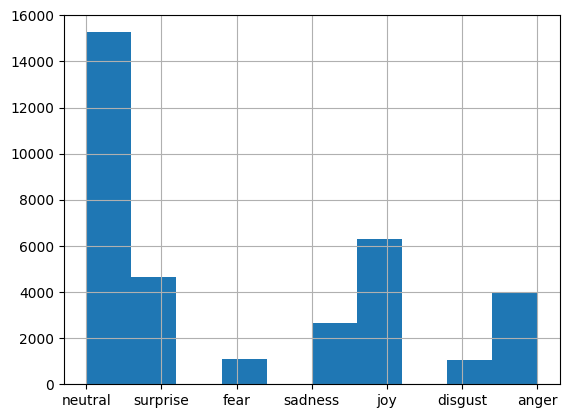
\includegraphics[width=0.48\textwidth]{img/em_dist.png}
    \caption{Emotions distribution in the dataset}
    \label{fig:em_dist}
    \centering
\end{figure}
Furthermore, 29425 sentences out of 35000 ($\sim$84.01\%) didn't cause an emotion flip in the conversation, meaning that the presence of positive triggers is quite rare.

One of the implemented systems performed an additional pre-processing step of the data, with the goal of improving the trigger prediction's F1 score. We extended the training set by using the \textbf{ContextualWordEmbsAug} class provided by the \textit{nlpaug} library. We created a pipeline of textual operations to be performed: insertion, swapping and random deletion of words. We also needed to specify the probability of the operation happening, and the Contextual Word Embedding that would be used by the class (bert-base-uncased). The insert and swap operators made use of context around words to add or swap them based on similarity.

Since we decided to encode the history, the current utterance, and the next one in the input for the BERT model, each one of these strings were augmented with the operations explained before.

The inputs of the augmentation pipeline were all the DataFrame's rows showing an emotion flip. For each of these training set sentences, we created and added two other similar variants, and tripled the support of emotion flip sentences in the training set. The validation and test splits remained untouched. An example of augmented utterance can be seen in  \autoref{tab:aug_example}.

\begin{table}[h]
    \centering
    \caption{Sentence augmentation example}
    \label{tab:aug_example}
    \begin{tabular}{|c|c|}
    \hline
    & sentence \\
    \hline
    original & Hi, listen, I'm sorry about before. \\
    aug 1 & hi, um listen, i'm sorry tonight. \\
    aug 2 & so hi, listen, i'm sorry earlier. \\
    \hline
    \end{tabular}
\end{table}


\attention{MAX 2 COLUMNS / 3 FOR COMBINED REPORTS. OMIT SECTION IN ASSIGNMENT REPORTS.}

\explanation{Provide a brief description of your data including some statistics and pointers (references to articles/URLs) to be used to obtain the data. Describe any pre-processing work you did. Links to datasets must be placed later in Section~\ref{sec:links}.}

\section{Experimental setup and results}
\label{sec:results}
\attention{MAX 1 COLUMN FOR ASSIGNMENT REPORTS / 3 COLUMNS FOR PROJECT OR PW / 5 FOR COMBINED REPORTS.}

\explanation{
Describe how you set up your experiments: which architectures/configurations you used, which hyper-parameters and what methods used to set them, which optimizers, metrics, etc.
\\
Then, \textbf{use tables} to summarize your your findings (numerical results) in validation and test. If you don't have experience with tables in \LaTeX, you might want to use \href{https://www.tablesgenerator.com/}{\LaTeX table generator} to quickly create a table template.
}

The execution and analysis of the model was performed using a python notebook which allowed to customize the hyper-parameters of the execution:

\begin{itemize}
    \item Learning rate: After some experimentation we settled to $5*10^{-5}$ as higher values cause worse performances
    \item Seed: a number to use as seed for pseudo-random number generation, pyTorch and CUDA. The five numbers chosen to be used as seeds were 11, 27, 35, 42 and 81.
    \item Weighted sampling: it is possible to enable or disable the usage of a weighted sampler in the training data loader (as described in section \ref{weighted_sampler})
    \item Trigger weight: number used as trigger loss scaling factor. We choose values equal or lower to 3 as higher values cause worse performance.
    \item Data augmentation: whether to perform data augmentation with nlpaug (as described in section \ref{nlpaug} and \ref{sec:data})
\end{itemize}

The notebook includes all the necessary steps for executing and evaluating the model:
\begin{itemize}
    \item Dataset ingestion, pre-processing, splitting and (if enabled) augmentation (as described in \ref{sec:system})
    %\item Exploratory Data Analysis % not highlighting it here as it is something we did before implementing the model
    \item Testing of the baseline model
    \item Training and testing of the model with the freezed base-model
    \item Training and testing of the model with the fully-finetuned model
    \item Programmatic error analysis on the output of the model
    \item Dump of the models' output and F1 scores to files for further manual analysis
\end{itemize}

For each model configuration tested we used as metrics the sequence F1 score (average of the dialogues' scores) and the unrolled sequence F1 score (average of the flattened utterances scores), for both emotions and triggers.

In order to prevent overtraining the models were trained with early stopping, halting training if the validation loss of an epoch is higher than the last.

Four combinations of hyper-parameters were chosen to test the model behavior:
\begin{itemize}
    \item S1: normal sampling, trigger weight = 3.0, no data augmentation
    \item S2: weighted sampling, trigger weight = 1.0, no data augmentation
    \item S3: normal sampling, trigger weight = 1.0, no data augmentation
    \item S4: normal sampling, trigger weight = 1.0, data augmentation enabled
\end{itemize}

The notebook was run for each combination of hyper-parameters and seed, with the results reported in \autoref{appendix_results}. A recap of F1 scores for triggers can be found in \autoref{tab:triggers_f1}.




\section{Discussion}
\subsection{Baselines}
Two baseline classifiers, namely the Random Classifier and the Majority Classifier, were employed in this study. The Random Classifier, owing to its inherent nature, serves as a weak benchmark for emotion classification, yielding an SEQ-F1 micro score of 0.150 for emotions and 0.510 for triggers. On the other hand, the Majority Classifier, which outputs the most frequent label, provides a more substantial baseline due to the imbalanced dataset. It achieves an SEQ-F1 micro score of 0.420 for emotions and a notably higher 0.809 for triggers.

The significance of the Majority Classifier as a baseline is particularly important as a reference, given the highly unbalanced nature of the dataset, in particular for the binary triggers classification. In binary classification, achieving a commendable F1 score can be relatively straightforward by consistently predicting the most frequent label (0). 

\subsection{BERT models results}
The Freezed and Full BERT models, configured with the initial settings (S3), demonstrated good performance in emotion classification and an equal performance in trigger classification, compared with the Majority Classifier. Moreover, we didn't notice a significant difference between the results of the Freezed and Full BERT models, with a slight advantage in favor of the Freezed BERT model. Consequently, in the following discussion it will be used as our trained model reference.

\subsubsection{Emotion Classification}
Both the Freezed and Full BERT models achieved really similar SEQ-F1 micro scores of 0.944 and 0.946, respectively. These scores represent a substantial improvement over the baseline models. As shown in \autoref{fig:cm_emo} the neutral label is the most accurately predicted, while anger, fear, sadness and disgust show a slightly higher miss-classification rate. This could be attributed to the imbalance of the dataset, without a particular pattern to be notice. In \autoref{fig:scatter} is possible to observe a correlation between the label support and the F1 score, which may explain the differences in scores, rather than an intrinsic label complexity. In fact, the neutral emotion, having the best support, exhibits the best F1 score, whereas disgust, anger and fear the lowest scores.

\begin{figure}[]
    \centering
    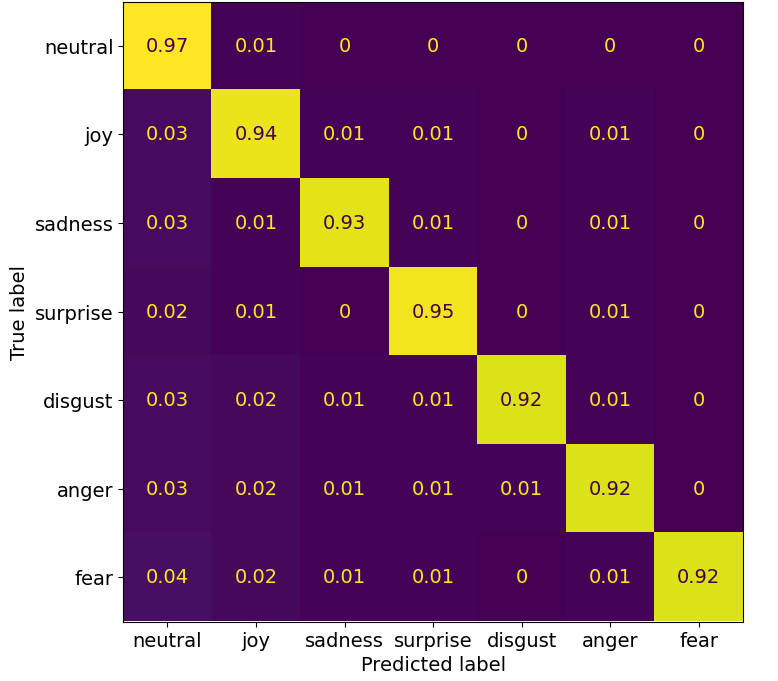
\includegraphics[width=0.48\textwidth]{img/cm_emo_S3.png}
    \caption{Emotion Classification, normalized confusion matrix - Freezed BERT, S3 settings}
    \label{fig:cm_emo}
    \centering
\end{figure}

\begin{figure}
    \centering
    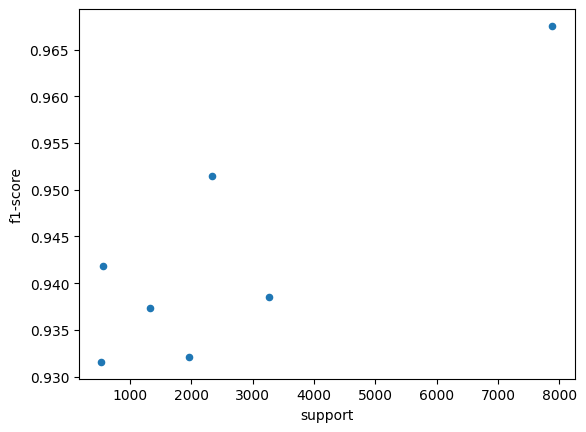
\includegraphics[width=0.48\textwidth]{img/scatter.png}
    \caption{F1 score and Support, Emotion Classification - Freezed BERT, S3 settings}
    \label{fig:scatter}
\end{figure}

\subsubsection{Trigger Classification}
On the contrary, when it comes to trigger classification, the models did not exhibit a significant enhancement compared to the Majority Classifier baseline, recording SEQ-F1 micro scores of 0.806 and 0.807. As shown in \autoref{fig:cm_tri} the Freezed BERT model demonstrated an high accuracy in the classification of sentences without a trigger. However, its capability in identifying triggers was notably low, with a tendency to miss-classify the presence of triggers in the majority of cases.

These similar performances between the trained models and the Majority Classifier may be attributed to the challenges posed by the highly imbalanced dataset and the inherent difficulty in identifying triggers within sentences. 

\subsubsection{Trigger Classification improvements}
Given the discussed results, we attempted various approaches in order to improve the trigger classification. \autoref{tab:triggers_f1} provides a comparison of the F1 scores for these attempts, while more detailed tables are presented in the Appendix.
\paragraph{S1 settings:} Our initial attempt involved assigning greater importance to the trigger loss during training. Both trained models exhibited a slight improvement in the F1 score for True triggers while maintaining the same score for False triggers classification. However, a minor decrease in the F1 score for emotion classification was observed. In summary, the overall triggers UNR-F1 and SEQ-F1 micro scores remained constant, with a slight improvement in the UNR-F1 macro scores.

\paragraph{S2 settings:} Moreover, we experimented the use of WeighterSampler to boost the trigger sentences' probability to be extracted. This approach led to a significant difference in the triggers F1 scores. Specifically, the False score declined from 0.913 to 0.776, but the True score had an important improvement, soaring from 0.132 to 0.296.
Consequently, both the UNR-F1 and SEQ-F1 micro score triggers score declined, but the UNR-F1 score macro slightly improved.

\paragraph{S4 settings:}Finally, we tried a data augmentation approach, with the purpose of increasing the sentences containing triggers in the dataset. However, this approach didn't led to any notably improvement in the outcome, resulting in a slightly worsening variation of the F1 score of the True trigger label.

\subsubsection{Encoding without the future sentence}
Initially we performed some tests by using a different encoding, that concatenated the \textit{history} and the current \textit{utterance}, without considering the \textit{future} sentence. That encoding was then changed, because including the future sentence improved the EFR task's Unrolled F1 Score macro by 2 points.


\begin{figure}[]
    \centering
    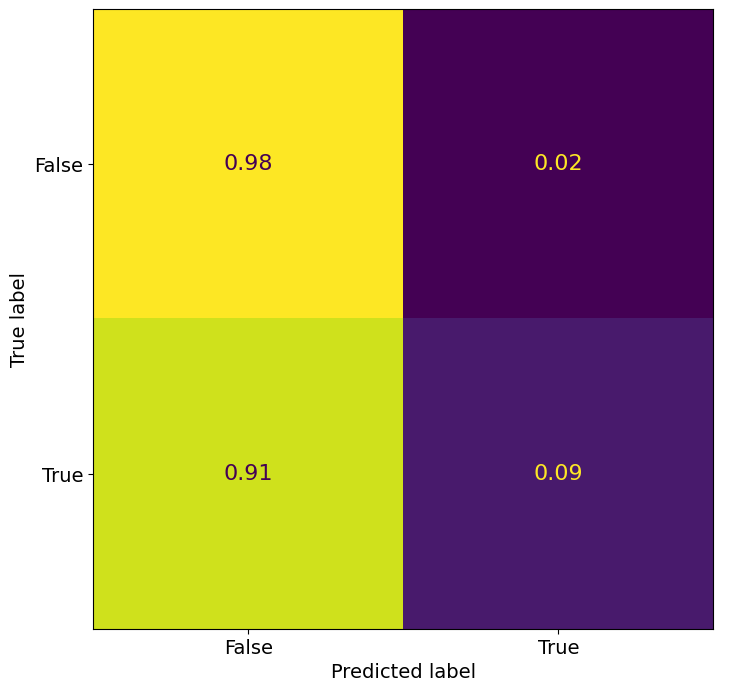
\includegraphics[width=0.48\textwidth]{img/cm_tri_S3.png}
    \caption{Trigger Classification, normalized confusion matrix - Freezed BERT, S3 settings}
    \label{fig:cm_tri}
    \centering
\end{figure}



\begin{table}[h]
    \centering
    \caption{Triggers F1 scores}
    \label{tab:triggers_f1}
    \begin{tabular}{|c|cc|cc|}
    \hline
                & \multicolumn{2}{c|}{Freezed BERT}  & \multicolumn{2}{c|}{Full BERT}     \\ \hline
    Trigger     & \multicolumn{1}{c|}{False}     & True    & \multicolumn{1}{c|}{False}     & True     \\ \hline
    \textbf{S1} & \multicolumn{1}{c|}{0.913} & 0.150 & \multicolumn{1}{c|}{0.913} & 0.171 \\ \hline
    \textbf{S2} & \multicolumn{1}{c|}{0.776} & 0.296 & \multicolumn{1}{c|}{0.789} & 0.289 \\ \hline
    \textbf{S3} & \multicolumn{1}{c|}{0.913} & 0.132 & \multicolumn{1}{c|}{0.912} & 0.148 \\ \hline
    \textbf{S4} & \multicolumn{1}{c|}{0.913} & 0.108 & \multicolumn{1}{c|}{0.912} & 0.104 \\ \hline
    \end{tabular}
\end{table}

\section{Conclusion}
\label{sec:conclusion}

This project explored and showed the performance of a BERT-based model for the ERC and EFR tasks, comparing it with a Random and a Majority Classifier baseline. Our model, trained on S3 settings, significantly improved the ERC task, compared to the two baselines. However, even if the SEQ-F1 and UNR-F1 for the emotion flip prediction improved significantly, it cannot be said to be good enough. 

Some tests based on different representations of the input were made to decide which sentences could provide a good enough context for both tasks, that resulted in the previously explained encoding (\textit{history+utterance [SEP] future-utterance}).

Our work then focused in finding alternative solutions for the model's training, with the goal of improving its emotion flip detection capabilities. The S1 and S2 solutions provided better EFR performance, at the cost of decreasing the emotion prediction's score. The S4 solution, using data augmentation to extend the dataset, proved to be not useful for this goal.

In conclusion, neither of the previous solutions let untouched the ERC performance while improving the EFR score. The most important findings that we obtained is about the input encoding. In fact, an encoding without the next sentence, resulted in having more or less the same scores in the ERC task, but worse performance for the EFR task.

Since the best improvement was obtained by changing the encoding, exploring more that subject could be useful for searching better solutions. Additional enhancements may involve experimenting with an expanded version of BERT or implementing distinguished BERT variants, such as RoBERTa or XLNet. 


\attention{MAX 1 COLUMN.}

\explanation{
In one or two paragraphs, recap your work and main results.
What did you observe? 
Did all go according to expectations? 
Was there anything surprising or worthwhile mentioning?
After that, discuss the main limitations of the solution you have implemented, and indicate promising directions for future improvement.
}



\section{Links to external resources}
\label{sec:links}
\begin{itemize}
    \item \href{https://drive.google.com/drive/folders/16mFdhXGECdcyDjLs_alI43W4iNQK_47B}{Dataset download} (Task 3 folder)
    \item \href{https://github.com/Danysan1/ai-unibo-nlp-project/tree/main/final}{Github Repository} with code. You should follow the \textit{execution.ipynb} Notebook.
    \item \href{https://netron.app/}{Netron App} was used to create an image of our model's classification heads.
    \item \href{https://colab.research.google.com/}{Google Colab} and \href{https://www.kaggle.com/code/}{Kaggle Notebooks} were used to run the code.
\end{itemize}

\attention{THIS SECTION IS OPTIONAL}
\explanation{
Insert here:
\begin{itemize}
    \item a link to your GitHub or any other public repo where one can find your code (only if you did not submit your code on Virtuale); 
    \item a link to your dataset (only for non-standard projects or project works).
\end{itemize}
}

\attention{DO NOT INSERT CODE IN THIS REPORT}


\bibliography{nlpreport.bib}


\onecolumn
%\section{Appendix Compressed}

\begin{table}[h]
\appendix
\section{Appendix}
\label{appendix_results}
\begin{tabular}{|l|cc|cc|}
\hline
\multicolumn{1}{|c|}{\textbf{Baseline}}              & \multicolumn{2}{c|}{Random}                                             & \multicolumn{2}{c|}{Majority}                                           \\ \hline
\multicolumn{1}{|c|}{}              & \multicolumn{1}{c|}{Average}                            & $\sigma$                         & \multicolumn{1}{c|}{Average}                            & $\sigma$                         \\ \hline
Sequence F1 emotions micro          & \multicolumn{1}{c|}{\cellcolor[HTML]{CB0000}0.150} & \cellcolor[HTML]{FFFFFF}0.004 & \multicolumn{1}{c|}{\cellcolor[HTML]{F8A102}0.430} & \cellcolor[HTML]{FFFFFF}0.007 \\ \hline
Sequence F1 triggers micro          & \multicolumn{1}{c|}{\cellcolor[HTML]{F8A102}0.510} & \cellcolor[HTML]{FFFFFF}0.008 & \multicolumn{1}{c|}{\cellcolor[HTML]{32CB00}0.809} & \cellcolor[HTML]{FFFFFF}0.012 \\ \hline
Unrolled Sequence F1 emotions micro & \multicolumn{1}{c|}{\cellcolor[HTML]{CB0000}0.147} & \cellcolor[HTML]{FFFFFF}0.004 & \multicolumn{1}{c|}{\cellcolor[HTML]{F8A102}0.441} & \cellcolor[HTML]{FFFFFF}0.010 \\ \hline
Unrolled Sequence F1 triggers micro & \multicolumn{1}{c|}{\cellcolor[HTML]{F8A102}0.507} & \cellcolor[HTML]{FFFFFF}0.006 & \multicolumn{1}{c|}{\cellcolor[HTML]{32CB00}0.847} & \cellcolor[HTML]{FFFFFF}0.010 \\ \hline
Unrolled Sequence F1 emotions macro & \multicolumn{1}{c|}{\cellcolor[HTML]{CB0000}0.123} & \cellcolor[HTML]{FFFFFF}0.003 & \multicolumn{1}{c|}{\cellcolor[HTML]{CB0000}0.087} & \cellcolor[HTML]{FFFFFF}0.001 \\ \hline
Unrolled Sequence F1 triggers macro & \multicolumn{1}{c|}{\cellcolor[HTML]{F8A102}0.437} & \cellcolor[HTML]{FFFFFF}0.008 & \multicolumn{1}{c|}{\cellcolor[HTML]{F8A102}0.458} & \cellcolor[HTML]{FFFFFF}0.003 \\ \hline
\end{tabular}

\bigskip
\begin{tabular}{|l|cc|cc|}
\hline
\multicolumn{1}{|c|}{\textbf{S1: trigger weight = 3.0}}              & \multicolumn{2}{c|}{BERT Full}                                                     & \multicolumn{2}{c|}{BERT Freezed}                                                  \\ \hline
\multicolumn{1}{|c|}{}              & \multicolumn{1}{c|}{Average}                       & $\sigma$                         & \multicolumn{1}{c|}{Average}                       & $\sigma$                         \\ \hline
Sequence F1 emotions micro          & \multicolumn{1}{c|}{\cellcolor[HTML]{009901}0.927} & \cellcolor[HTML]{FFFFFF}0.022 & \multicolumn{1}{c|}{\cellcolor[HTML]{009901}0.931} & \cellcolor[HTML]{FFFFFF}0.001 \\ \hline
Sequence F1 triggers micro          & \multicolumn{1}{c|}{\cellcolor[HTML]{34FF34}0.809} & \cellcolor[HTML]{FFFFFF}0.016 & \multicolumn{1}{c|}{\cellcolor[HTML]{34FF34}0.808} & \cellcolor[HTML]{FFFFFF}0.010 \\ \hline
Unrolled Sequence F1 emotions micro & \multicolumn{1}{c|}{\cellcolor[HTML]{009901}0.936} & \cellcolor[HTML]{FFFFFF}0.018 & \multicolumn{1}{c|}{\cellcolor[HTML]{009901}0.941} & \cellcolor[HTML]{FFFFFF}0.003 \\ \hline
Unrolled Sequence F1 triggers micro & \multicolumn{1}{c|}{\cellcolor[HTML]{34FF34}0.842} & \cellcolor[HTML]{FFFFFF}0.013 & \multicolumn{1}{c|}{\cellcolor[HTML]{34FF34}0.843} & \cellcolor[HTML]{FFFFFF}0.009 \\ \hline
Unrolled Sequence F1 emotions macro & \multicolumn{1}{c|}{\cellcolor[HTML]{009901}0.917} & \cellcolor[HTML]{FFFFFF}0.026 & \multicolumn{1}{c|}{\cellcolor[HTML]{009901}0.924} & \cellcolor[HTML]{FFFFFF}0.003 \\ \hline
Unrolled Sequence F1 triggers macro & \multicolumn{1}{c|}{\cellcolor[HTML]{F8A102}0.541} & \cellcolor[HTML]{FFFFFF}0.015 & \multicolumn{1}{c|}{\cellcolor[HTML]{F8A102}0.531} & \cellcolor[HTML]{FFFFFF}0.015 \\ \hline
\end{tabular}

\bigskip
\begin{tabular}{|l|cc|cc|}
\hline
\multicolumn{1}{|c|}{\textbf{S2: weighted sampling}}              & \multicolumn{2}{c|}{BERT Full}                                                     & \multicolumn{2}{c|}{BERT Freezed}                                                  \\ \hline
\multicolumn{1}{|c|}{}              & \multicolumn{1}{c|}{Average}                       & $\sigma$                         & \multicolumn{1}{c|}{Average}                       & $\sigma$                         \\ \hline
Sequence F1 emotions micro          & \multicolumn{1}{c|}{\cellcolor[HTML]{009901}0.916} & \cellcolor[HTML]{FFFFFF}0.017 & \multicolumn{1}{c|}{\cellcolor[HTML]{009901}0.921} & \cellcolor[HTML]{FFFFFF}0.007 \\ \hline
Sequence F1 triggers micro          & \multicolumn{1}{c|}{\cellcolor[HTML]{D3F008}0.667} & \cellcolor[HTML]{FFFFFF}0.018 & \multicolumn{1}{c|}{\cellcolor[HTML]{D3F008}0.656} & \cellcolor[HTML]{FFFFFF}0.008 \\ \hline
Unrolled Sequence F1 emotions micro & \multicolumn{1}{c|}{\cellcolor[HTML]{009901}0.926} & \cellcolor[HTML]{FFFFFF}0.015 & \multicolumn{1}{c|}{\cellcolor[HTML]{009901}0.932} & \cellcolor[HTML]{FFFFFF}0.005 \\ \hline
Unrolled Sequence F1 triggers micro & \multicolumn{1}{c|}{\cellcolor[HTML]{D3F008}0.674} & \cellcolor[HTML]{FFFFFF}0.016 & \multicolumn{1}{c|}{\cellcolor[HTML]{D3F008}0.660} & \cellcolor[HTML]{FFFFFF}0.009 \\ \hline
Unrolled Sequence F1 emotions macro & \multicolumn{1}{c|}{\cellcolor[HTML]{009901}0.907} & \cellcolor[HTML]{FFFFFF}0.020 & \multicolumn{1}{c|}{\cellcolor[HTML]{009901}0.916} & \cellcolor[HTML]{FFFFFF}0.004 \\ \hline
Unrolled Sequence F1 triggers macro & \multicolumn{1}{c|}{\cellcolor[HTML]{F8A102}0.538} & \cellcolor[HTML]{FFFFFF}0.008 & \multicolumn{1}{c|}{\cellcolor[HTML]{F8A102}0.536} & \cellcolor[HTML]{FFFFFF}0.008 \\ \hline
\end{tabular}

\bigskip
\begin{tabular}{|l|cc|cc|}
\hline
\multicolumn{1}{|c|}{\textbf{S3: standard}}              & \multicolumn{2}{c|}{BERT Full}                                                     & \multicolumn{2}{c|}{BERT Freezed}                                                  \\ \hline
\multicolumn{1}{|c|}{}              & \multicolumn{1}{c|}{Average}                       & $\sigma$                         & \multicolumn{1}{c|}{Average}                       & $\sigma$                         \\ \hline
Sequence F1 emotions micro          & \multicolumn{1}{c|}{\cellcolor[HTML]{009901}0.944} & \cellcolor[HTML]{FFFFFF}0.006 & \multicolumn{1}{c|}{\cellcolor[HTML]{009901}0.946} & \cellcolor[HTML]{FFFFFF}0.007 \\ \hline
Sequence F1 triggers micro          & \multicolumn{1}{c|}{\cellcolor[HTML]{32CB00}0.806} & \cellcolor[HTML]{FFFFFF}0.011 & \multicolumn{1}{c|}{\cellcolor[HTML]{32CB00}0.807} & \cellcolor[HTML]{FFFFFF}0.011 \\ \hline
Unrolled Sequence F1 emotions micro & \multicolumn{1}{c|}{\cellcolor[HTML]{009901}0.952} & \cellcolor[HTML]{FFFFFF}0.004 & \multicolumn{1}{c|}{\cellcolor[HTML]{009901}0.953} & \cellcolor[HTML]{FFFFFF}0.005 \\ \hline
Unrolled Sequence F1 triggers micro & \multicolumn{1}{c|}{\cellcolor[HTML]{32CB00}0.841} & \cellcolor[HTML]{FFFFFF}0.008 & \multicolumn{1}{c|}{\cellcolor[HTML]{32CB00}0.842} & \cellcolor[HTML]{FFFFFF}0.009 \\ \hline
Unrolled Sequence F1 emotions macro & \multicolumn{1}{c|}{\cellcolor[HTML]{009901}0.943} & \cellcolor[HTML]{FFFFFF}0.008 & \multicolumn{1}{c|}{\cellcolor[HTML]{009901}0.942} & \cellcolor[HTML]{FFFFFF}0.008 \\ \hline
Unrolled Sequence F1 triggers macro & \multicolumn{1}{c|}{\cellcolor[HTML]{F8A102}0.529} & \cellcolor[HTML]{FFFFFF}0.019 & \multicolumn{1}{c|}{\cellcolor[HTML]{F8A102}0.522} & \cellcolor[HTML]{FFFFFF}0.022 \\ \hline
\end{tabular}

\bigskip
\begin{tabular}{|l|cc|cc|}
\hline
\multicolumn{1}{|c|}{\textbf{S4: with data augmentation}}              & \multicolumn{2}{c|}{BERT Full}                                                     & \multicolumn{2}{c|}{BERT Freezed}                                                  \\ \hline
\multicolumn{1}{|c|}{}              & \multicolumn{1}{c|}{Average}                       & $\sigma$                         & \multicolumn{1}{c|}{Average}                       & $\sigma$                         \\ \hline
Sequence F1 emotions micro          & \multicolumn{1}{c|}{\cellcolor[HTML]{009901}0.935} & \cellcolor[HTML]{FFFFFF}0.009 & \multicolumn{1}{c|}{\cellcolor[HTML]{009901}0.942} & \cellcolor[HTML]{FFFFFF}0.004 \\ \hline
Sequence F1 triggers micro          & \multicolumn{1}{c|}{\cellcolor[HTML]{32CB00}0.803} & \cellcolor[HTML]{FFFFFF}0.011 & \multicolumn{1}{c|}{\cellcolor[HTML]{32CB00}0.806} & \cellcolor[HTML]{FFFFFF}0.014 \\ \hline
Unrolled Sequence F1 emotions micro & \multicolumn{1}{c|}{\cellcolor[HTML]{009901}0.944} & \cellcolor[HTML]{FFFFFF}0.008 & \multicolumn{1}{c|}{\cellcolor[HTML]{009901}0.951}  & \cellcolor[HTML]{FFFFFF}0.002 \\ \hline
Unrolled Sequence F1 triggers micro & \multicolumn{1}{c|}{\cellcolor[HTML]{32CB00}0.839} & \cellcolor[HTML]{FFFFFF}0.010 & \multicolumn{1}{c|}{\cellcolor[HTML]{32CB00}0.842} & \cellcolor[HTML]{FFFFFF}0.011 \\ \hline
Unrolled Sequence F1 emotions macro & \multicolumn{1}{c|}{\cellcolor[HTML]{009901}0.932} & \cellcolor[HTML]{FFFFFF}0.010 & \multicolumn{1}{c|}{\cellcolor[HTML]{009901}0.940} & \cellcolor[HTML]{FFFFFF}0.005 \\ \hline
Unrolled Sequence F1 triggers macro & \multicolumn{1}{c|}{\cellcolor[HTML]{F8A102}0.507} & \cellcolor[HTML]{FFFFFF}0.018 & \multicolumn{1}{c|}{\cellcolor[HTML]{F8A102}0.511} & \cellcolor[HTML]{FFFFFF}0.018 \\ \hline
\end{tabular}
\end{table}


\end{document}